\chapter{Project Reflection \\
  \small{\textit{-- Evan Ciok, Sophia DiCuffa, Carson McManus}}
  \label{Chapter::ProjectReflection}}

\section{Issue Tracking}

See issue tracking here: \href{https://github.com/users/dyc3/projects/2/views/1}{https://github.com/users/dyc3/projects/2/views/1}

\begin{figure}
	\centering
	\scalebox{0.25}{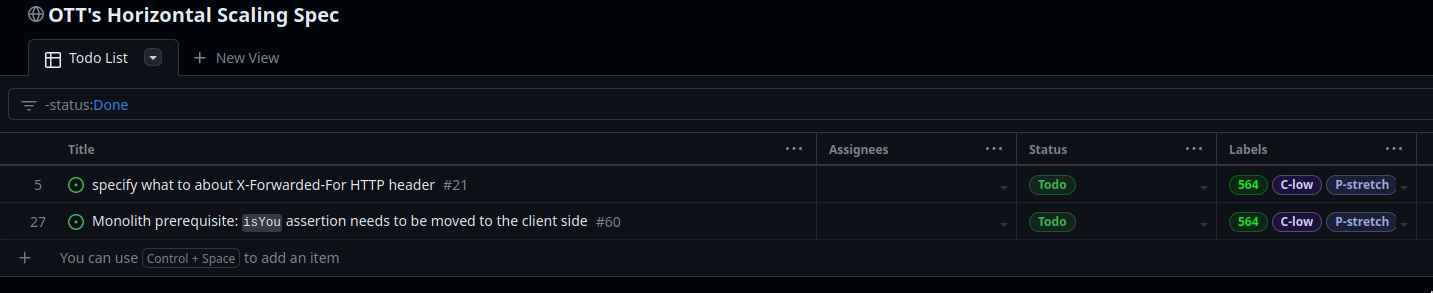
\includegraphics{Figures/gh-incomplete.png}}
	\caption{\label{Figure::gh-incomplete} Incomplete issues.}
\end{figure}

\begin{figure}
	\centering
	\scalebox{0.25}{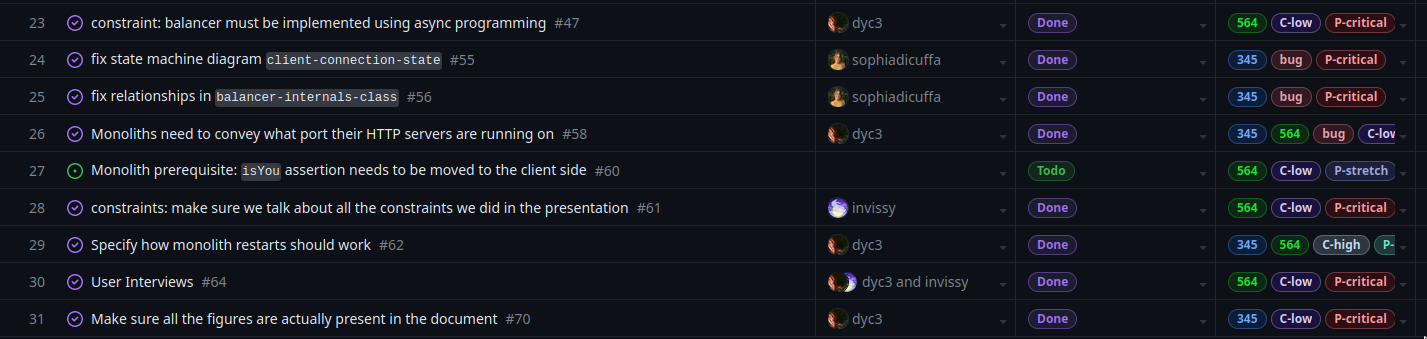
\includegraphics{Figures/gh-issue-sample.png}}
	\caption{\label{Figure::gh-issue-sample.png} A sample of our issue tracking}
\end{figure}

\section{Process Reflection}

We probably would have benefitted from making more progress earlier, and from more consistent meetings.

\subsection{Agile Process}

The agile process was not strictly followed. There are no meeting notes (which were not required when we started working on the project). Instead, all outcomes from meetings are reflected in opened issues.

\section{Group Effort (only for ssw-345 paper requirements)}

\begin{itemize}
	\item Carson: 50\% - Put in majority effort, mostly out of necessity to effectively communicate the project to the rest of the group.
	\item Sophia: 25\% - Put in good effort to specify the API proxy, and to make diagrams.
	\item Evan: 25\% - Put in good effort to specify maintaining room states, and to make diagrams.
\end{itemize}